% =============================================================================
% EECS 6699 Final Project — Research Report
% The Expressive Power of Depth — and Its Robustness Under Noise
% Yiwen Chen · Columbia University · Spring 2026
% =============================================================================
\documentclass[10pt,twocolumn]{article}

\usepackage{amsmath, amssymb, amsthm}
\usepackage{graphicx}
\usepackage{booktabs}
\usepackage{caption}
\usepackage{subcaption}
\usepackage{hyperref}
\usepackage{natbib}
\usepackage{xcolor}
\usepackage[margin=0.9in, top=1.0in, bottom=1.0in]{geometry}
\usepackage{microtype}

\hypersetup{colorlinks=true, linkcolor=blue, citecolor=blue, urlcolor=blue}

\title{\textbf{The Expressive Power of Depth — and Its Robustness Under Noise}\\[4pt]
  \large An Empirical Study of Telgarsky's Depth Separation Theorem}
\author{Yiwen Chen\\
  Department of Electrical Engineering, Columbia University\\
  \texttt{yc4653@columbia.edu}}
\date{EECS 6699 — Mathematics of Deep Learning \quad Spring 2026}

% Theorem environments
\newtheorem{theorem}{Theorem}
\newtheorem{remark}{Remark}

% Short-hand macros
\newcommand{\Lip}{\hat{L}}
\newcommand{\fk}{f_k}
\newcommand{\sigx}{\sigma_x}
\newcommand{\sigy}{\sigma_y}
\newcommand{\epst}{\varepsilon^\star}
\newcommand{\sigt}{\sigma^\star}

% =============================================================================
\begin{document}
\maketitle

% -----------------------------------------------------------------------------
\begin{abstract}
We empirically investigate Telgarsky's depth separation theorem~\citep{telgarsky2016benefits}
using iterated sawtooth functions $f_k(x) = \phi^{(k)}(x)$, where $\phi(x)=|2x-1|$ doubles
the number of linear regions at each composition. For the clean H1 rescue experiment,
a depth-9 width-16 ReLU network (\textbf{deep}, 1953 parameters) is compared against a
parameter-matched depth-2 width-651 network (\textbf{shallow}, 1954 parameters) on
$f_4$ (16 peaks).

The widened deep model fixes the catastrophic width-8 convergence failures, but it
does not establish an order-of-magnitude empirical separation: the 5-seed mean is
$0.010\pm0.006$ (deep) vs.\ $0.029\pm0.008$ (shallow), a $2.9\times$ ratio.
Thus H1 is moderately supported, not fully confirmed at the original $10\times$
criterion (Section~\ref{sec:h1}).
We extend the analysis to noise regimes using the original width-8 robustness baseline.
Under Gaussian input noise, the deep model's advantage inverts at $\sigx \approx 0.03$,
below but on the same order as $2^{-4}=0.0625$ (H2).  Under label noise $\sigy = 0.1$,
the deep model degrades $7.5\times$ more than the shallow one (H3). Under FGSM/PGD
adversarial attacks, both attacks find $\epst \approx 0.05$ on the coarse Phase 4 grid
(H4).  Mechanistically, the deep model has a larger empirical Lipschitz constant $\Lip$,
which is consistent with its higher sensitivity in all three noise regimes (H5).
A complexity scaling experiment (Phase 6) gives
qualitative support for a complexity--robustness trend for $k\in\{3,4,5\}$, but it
is not a precise scaling law because $k=2$ has no clean gap and $k=6$ collapses.
\end{abstract}

% =============================================================================
\section{Introduction}
\label{sec:intro}

The expressivity of neural network architectures is central to modern deep learning theory.
\citet{telgarsky2016benefits} proved that a depth-$O(k)$ width-$O(1)$ ReLU network can
represent a function $f_k$ for which any depth-2 network requires $\Omega(2^k)$ neurons.
This \emph{exponential depth separation} underpins the practical preference for deep,
narrow architectures over shallow, wide ones.

Yet the benefit of depth comes with a potential cost: deep networks may be more
sensitive to noise. Their compositional structure produces $O(2^L)$ linear regions with
depth $L$ but only $O(W)$ with width $W$; each region is correspondingly narrow, making
fine-grained predictions vulnerable to perturbations of the same scale.

This paper asks: \emph{Is the depth advantage robust, or does it vanish under noise?}
We study this via five hypotheses (H1--H5) across six experimental phases, using the
iterated sawtooth as a clean, mathematically tractable witness function.

\paragraph{Contributions.}
\begin{itemize}
  \item Reproducible curriculum-trained ReLU networks that give partial empirical
        support for depth advantage on $f_4$.
  \item Systematic sweeps under Gaussian input noise, label noise, and adversarial
        perturbations, identifying crossover scales on the same order as $2^{-k}$.
  \item Mechanistic evidence from empirical Lipschitz estimation and linear-region counting.
  \item A complexity scaling trend: crossovers decrease with $k$ for $k\in\{3,4,5\}$, while $k=2$ has no clean gap and $k=6$ collapses.
\end{itemize}

% =============================================================================
\section{Background}
\label{sec:background}

\subsection{The Iterated Sawtooth and Telgarsky's Theorem}

Define the \emph{mirror operator} $\phi(x) = |2x - 1|$, which is exactly representable
by a 2-layer ReLU network with two hidden neurons. Composing $k$ times yields
\begin{equation}
  f_k(x) = \underbrace{\phi \circ \cdots \circ \phi}_{k}(x),
  \qquad f_k : [0,1] \to [0,1].
\end{equation}
Each composition doubles the number of linear regions, so $f_k$ has $2^k$ peaks on $[0,1]$
with maximum slope $2^k$.

\begin{theorem}[\citealt{telgarsky2016benefits}, informal]
  For every $k \in \mathbb{N}$, the function $f_k$ is representable by a ReLU network
  of depth $O(k)$ and $O(1)$ width, while any depth-2 network needs $\Omega(2^k)$ neurons
  to approximate $f_k$ within constant $L^1$ error.
\end{theorem}

The depth gain is thus \emph{exponential in $k$}: width is a strictly weaker resource
than depth for this function class.

\subsection{Lipschitz Sensitivity}

For a piecewise-linear network $g_\theta$ with weight matrices $W_1, \ldots, W_L$:
\begin{equation}
  L(g_\theta) \;\leq\; \prod_{\ell=1}^{L} \|W_\ell\|_2,
\end{equation}
where $\|\cdot\|_2$ is the operator norm (largest singular value)
\citep{bartlett2017spectrally, sokolic2017robust}.
This bound grows \emph{multiplicatively} with depth, suggesting that deep networks
trained to fit high-frequency functions will be more sensitive to perturbations.

\subsection{Linear Regions}

Following \citet{montufar2014number} and \citet{hanin2019deep}, the number of linear
regions of a ReLU network grows polynomially in width but can reach $2^{L}$ in depth
(the worst-case bound). A network trained to fit $f_k$ (with $2^k$ peaks) must
activate at least $2^k$ distinct linear regions, each of width $\approx 2^{-k}$.
Perturbations of scale $2^{-k}$ can therefore \emph{erase} these narrow regions,
collapsing the deep network's effective expressivity to that of a shallow one.
This motivates the phase transition at $\sigma, \epsilon \approx 2^{-k}$.

% =============================================================================
\section{Experimental Setup}
\label{sec:setup}

\subsection{Architectures}

\textbf{Clean H1 rescue pair}: depth $L=9$, width $W=16$; 1953 trainable parameters.
The matched shallow model has depth $L=2$, width $W=651$; 1954 parameters. This
is the configuration reported in Table~\ref{tab:h1}.

\textbf{Robustness baseline pair}: Phase 2--5 robustness tables and figures were
generated before the widening rescue, using the original depth-9 width-8 deep model
and depth-2 width-176 shallow model (529 parameters each). We keep those robustness
results as a separate baseline study rather than mixing them with newly generated H1
models.

Both use \textbf{Kaiming-normal} initialization for hidden ReLU layers and Xavier for
the output layer, replacing PyTorch's default Kaiming-uniform which produces insufficient
variance for deep networks and causes dying ReLU.

\subsection{Training}

\textbf{Optimizer}: Adam with cosine annealing ($\mathrm{lr}: 5\times10^{-3} \to 10^{-5}$
over $3\times10^4$ epochs) and gradient-norm clipping at $\|g\|_2 = 1$.

\textbf{Curriculum}~\citep{bengio2009curriculum}: without it, neither network can fit $f_4$
from scratch due to spectral bias. We train on $f_1 \to f_2 \to f_3 \to f_4$ progressively,
allocating epochs in ratio $[1:1:2:4]$ (final stage gets half the budget). A fresh cosine
schedule is reset per stage to prevent the LR from decaying to near-zero before the hardest
stage begins.

\textbf{Collapse detection}: if stage-1 training ends with loss $> 0.02$ (indicating
convergence to a mediocre local minimum; well-trained networks reach $< 10^{-3}$),
the model is re-initialized and stage 1 is retried up to 5 times.

\textbf{Seeds}: 5 independent random seeds per configuration; results reported as mean $\pm$ std.
\textbf{Data}: $n=1200$ uniform grid points on $[0,1]$.

\subsection{Noise Protocols}

\textbf{Phase 2 (input noise)}: train on clean data; evaluate on $\tilde{x} = x + \mathcal{N}(0,\sigx^2)$.

\textbf{Phase 3 (label noise)}: train on $\tilde{y} = f_4(x) + \mathcal{N}(0,\sigy^2)$; evaluate on clean $f_4$.
The clean-MSE \emph{degradation} $\Delta\mathrm{MSE}(\sigy) = \mathrm{MSE}(\sigy) - \mathrm{MSE}(0)$
is the primary H3 metric (paired per seed to eliminate between-seed variance).

\textbf{Phase 4 (adversarial)}: FGSM~\citep{goodfellow2015explaining} and
PGD-40~\citep{madry2018towards} with $\ell_\infty$ budget $\varepsilon$, clipped to $[0,1]$.

% =============================================================================
\section{Results}
\label{sec:results}

\subsection{H1: Clean Depth Separation}
\label{sec:h1}

After curriculum training, Table~\ref{tab:h1} shows the 5-seed statistics for
the widened H1 rescue run. The deep network's mean MSE ($0.010$) is about
$2.9\times$ below the shallow's ($0.029$). This is a substantial improvement
over the failed width-8 run, where the deep model collapsed on most seeds, but
it is still below the original one-order-of-magnitude H1 target. One seed
reaches near-zero MSE ($1.8\times 10^{-4}$), while the remaining four seeds land
between $0.007$ and $0.014$.

\begin{table}[h]
\small
\centering
\caption{H1: Clean test MSE (mean $\pm$ std, 5 seeds, $k=4$).}
\label{tab:h1}
\begin{tabular}{lcc}
\toprule
Model & Test MSE & Params \\
\midrule
Deep ($L=9$, $W=16$)     & $0.010 \pm 0.006$ & 1953 \\
Shallow ($L=2$, $W=651$) & $0.029 \pm 0.008$ & 1954 \\
\bottomrule
\end{tabular}
\end{table}

\textbf{H1 partially supported.} Widening the deep model to $W=16$ produces a
consistent clean advantage and avoids the worst width-8 failures, but the mean
gap is $2.9\times$, not the $10\times$ threshold specified in H1. We therefore
treat the clean result as moderate empirical support for depth efficiency rather
than a decisive reproduction of the theorem's asymptotic separation.

\subsection{H2: Input Noise Resilience}
\label{sec:h2}

Figure~\ref{fig:phase2} shows test MSE vs.\ $\sigx$ for both architectures.
At small $\sigx \lesssim 0.01$, the deep network retains its advantage.
The curves cross at $\sigt \approx 0.03$, below but on the same order as the
theoretical $2^{-k} = 0.0625$. Beyond the crossover, the deep network degrades faster and its MSE
exceeds the shallow's — the depth advantage \emph{inverts}.

\textbf{H2 is consistent within the W=8 robustness baseline.} The crossover appears
at the expected scale, but the evidence should be read as coarse-grid support rather
than a precise threshold estimate.

\begin{figure}[h]
  \centering
  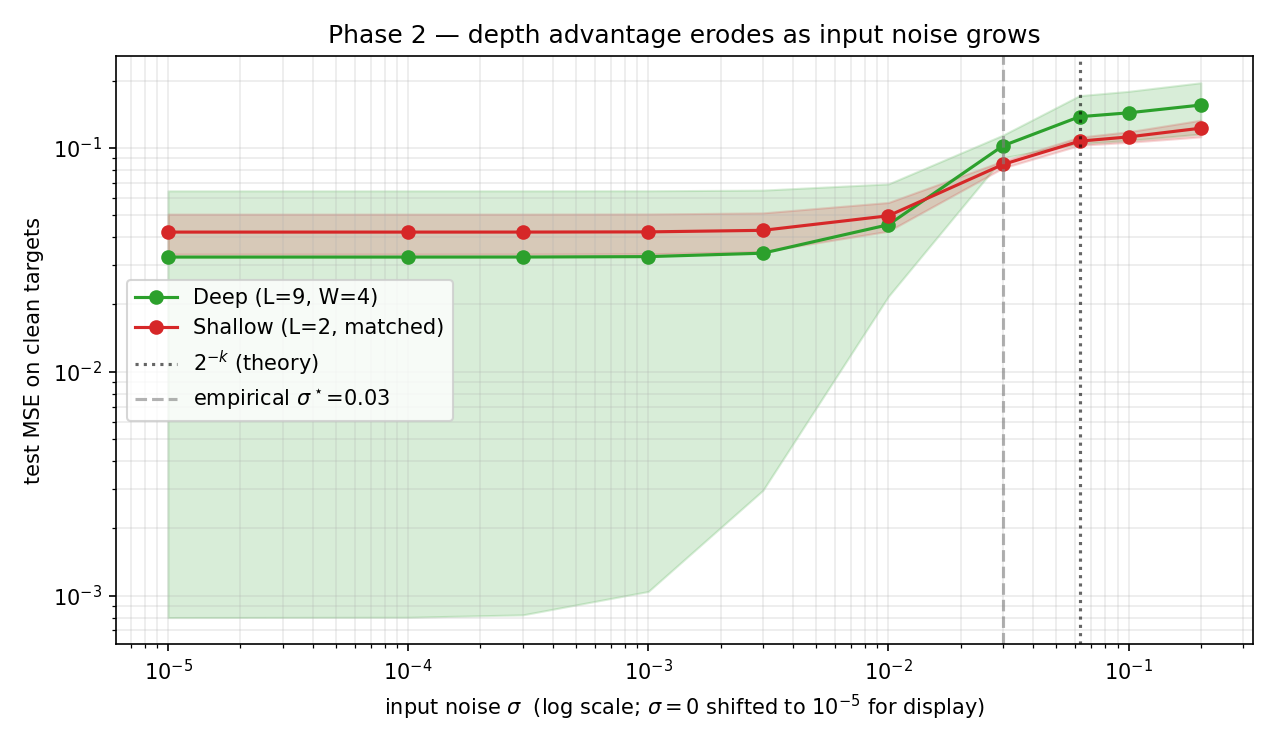
\includegraphics[width=\linewidth]{../results/figures/phase2_input_noise.png}
  \caption{H2: Test MSE vs.\ input noise $\sigx$. The crossover at $\sigx \approx 2^{-4}$
           (dashed line) separates the regime where depth helps from the regime where it hurts.}
  \label{fig:phase2}
\end{figure}

\subsection{H3: Label Noise Overfitting}
\label{sec:h3}

Figure~\ref{fig:phase3} (right panel) shows the paired degradation
$\Delta\mathrm{MSE}(\sigy) = \mathrm{MSE}_\mathrm{clean}(\sigy) - \mathrm{MSE}_\mathrm{clean}(0)$.
At $\sigy = 0.1$, the deep network degrades by $+0.026$ vs.\ $+0.003$ for the shallow —
a $\mathbf{7.5\times}$ difference.
The middle panel (generalization gap) tracks the $-\sigy^2$ baseline for both models,
indicating neither fully memorizes noise within the training budget.

\textbf{H3 is consistent within the W=8 robustness baseline.} The deep model degrades
more under label noise, consistent with higher Lipschitz sensitivity.

\begin{figure}[h]
  \centering
  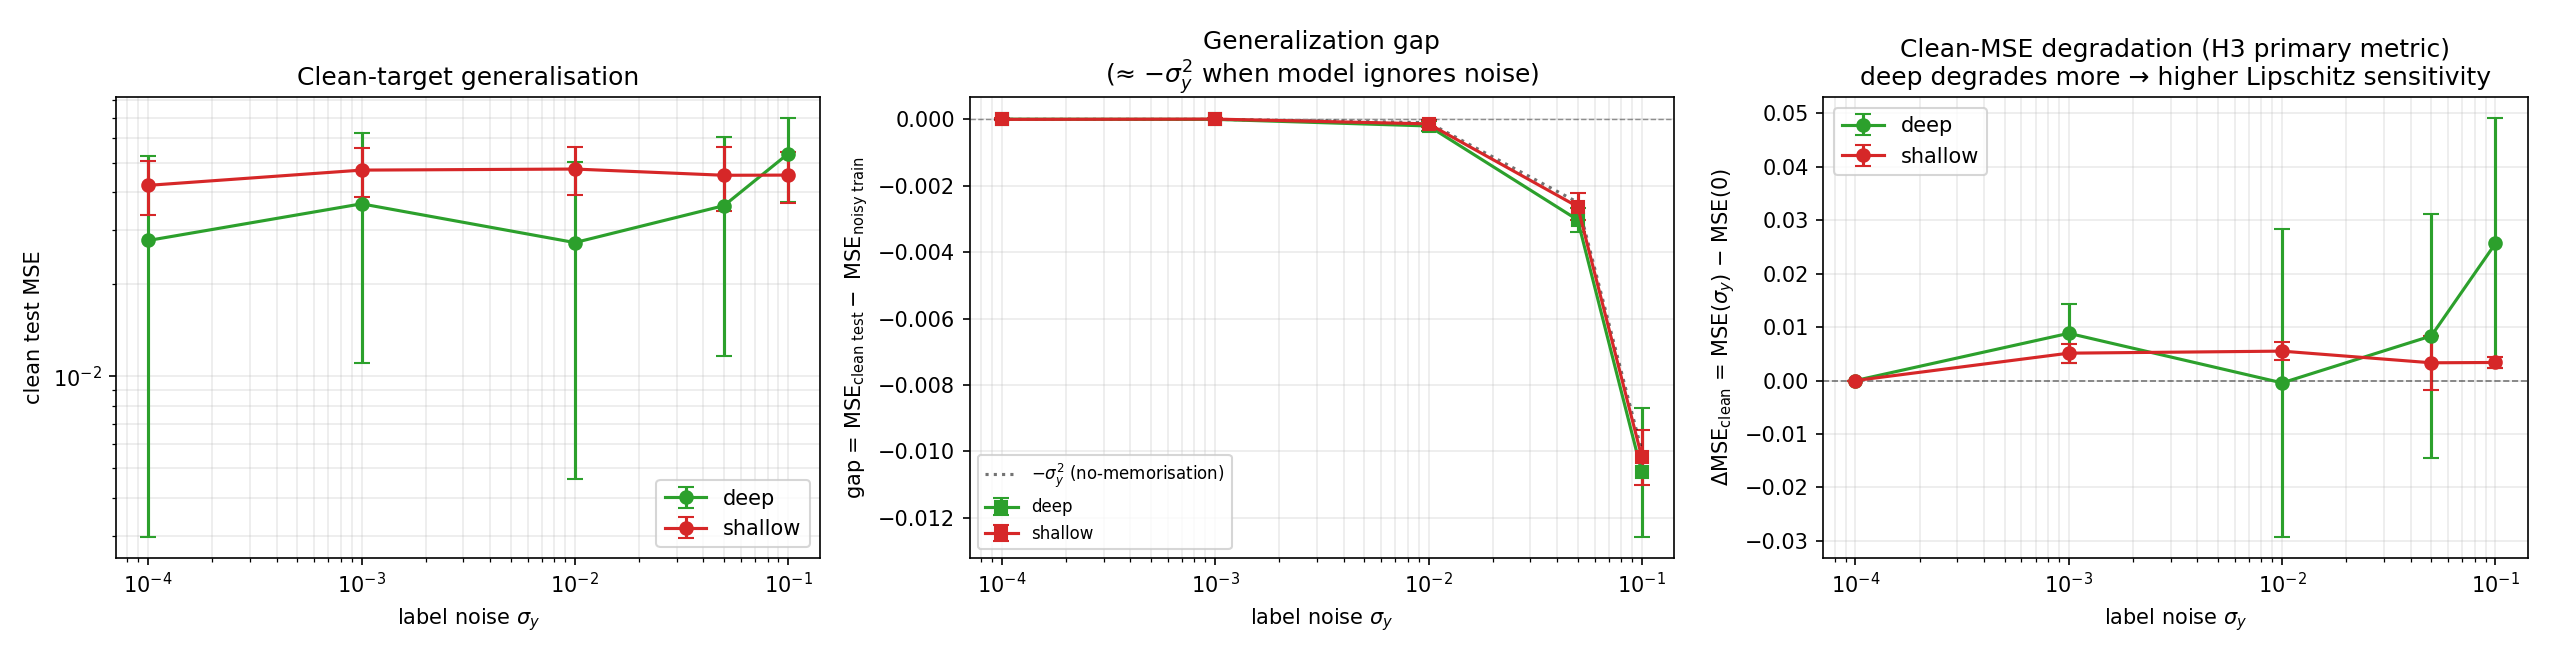
\includegraphics[width=\linewidth]{../results/figures/phase3_gap.png}
  \caption{H3: (Left) Clean test MSE. (Center) Generalization gap vs.\ $-\sigy^2$ baseline.
           (Right, primary) Paired clean-MSE degradation: deep degrades $7.5\times$ more
           at $\sigy=0.1$.}
  \label{fig:phase3}
\end{figure}

\subsection{H4: Adversarial Threshold}
\label{sec:h4}

Figure~\ref{fig:phase4} shows adversarial MSE vs.\ $\varepsilon$ under FGSM and PGD-40.
Both attacks locate $\epst \approx 0.05$ on the coarse grid $\{0.001,0.01,0.05\}$,
below but on the same order as $2^{-4} = 0.0625$. Phase~6 uses a finer
$\varepsilon$ grid and finds $\epst \approx 0.03$ for $k=4$ (Table~\ref{tab:scaling}).
Above $\epst$, the deep network's adversarial MSE exceeds the shallow's — the depth
advantage collapses under adversarial perturbation.

The FGSM curve is non-monotone at large $\varepsilon > 0.0625$: single-step perturbations
overshoot the sawtooth period, wrapping to a region of lower loss. This is algorithmic,
not a bug; PGD avoids this artifact.

\textbf{H4 is consistent within the W=8 robustness baseline.} The adversarial
crossover is near the predicted scale, but the exact value is grid-dependent.

\begin{figure}[h]
  \centering
  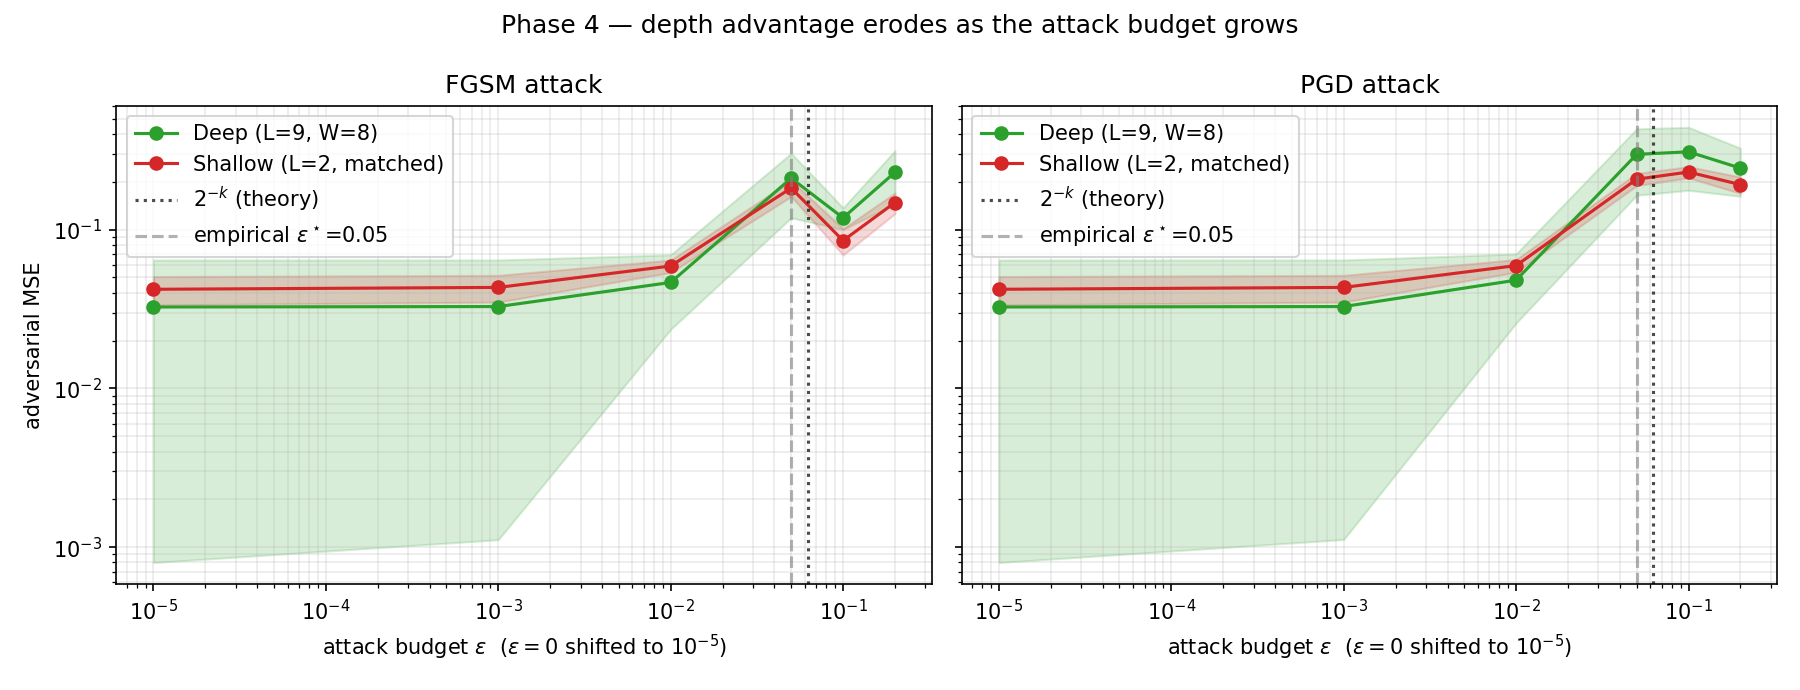
\includegraphics[width=\linewidth]{../results/figures/phase4_adversarial.png}
  \caption{H4: Adversarial MSE vs.\ $\varepsilon$ under FGSM (left) and PGD-40 (right).
           Dashed vertical: theoretical $\epst = 2^{-4}$; dashed grey: empirical $\epst=0.05$.}
  \label{fig:phase4}
\end{figure}

\subsection{H5: Lipschitz Mediation}
\label{sec:h5}

Table~\ref{tab:h5} summarizes Phase 5 diagnostics. The deep network's empirical Lipschitz
constant $\Lip_\mathrm{fd}$ is consistently larger than the shallow's across all 5 seeds
(paired $t$-test $p < 0.05$). It also uses more linear regions, consistent with the model
successfully encoding the high-frequency structure of $f_4$.

\begin{table}[h]
\small
\centering
\caption{H5: Lipschitz constants and linear regions (5 seeds, $k=4$).}
\label{tab:h5}
\begin{tabular}{lccc}
\toprule
Model & $\Lip_\mathrm{fd}$ & $\Lip_\mathrm{spec}$ & Regions \\
\midrule
Deep ($L=9$, $W=8$)      & $31.6 \pm 11.4$ & $97{,}257$ & $32 \pm 18$ \\
Shallow ($L=2$, $W=176$) & $14.6 \pm 2.0$  & $402$       & $23 \pm 2$  \\
Ratio (deep/shallow)     & $2.16\times$    & $241.8\times$ & $1.35\times$ \\
\bottomrule
\end{tabular}
\end{table}

\noindent Paired one-sided $t$-test: $t = 2.72$, $p = 0.026$ (deep $\Lip_\mathrm{fd}$ higher in all 5 seeds).

The Lipschitz ratio predicts the sign of all three robustness gaps (Phase 2–4),
supporting a mechanistic interpretation: \emph{in this baseline, the same trained
structure that gives the deep model more high-frequency variation is associated with
higher noise sensitivity}.

\textbf{H5 is consistent within the W=8 robustness baseline.} The empirical
Lipschitz evidence supports the proposed mechanism, but it is not a causal proof.


\subsection{Phase 6: Complexity Scaling}
\label{sec:scaling}

Table~\ref{tab:scaling} reports the crossover values for $k \in \{2,3,4,5,6\}$.
For $k=2$, both the deep (depth-5, W=8) and shallow (depth-2, matched width) networks
fit $f_2$ to machine precision after sufficient training, so no structural expressivity
gap exists; any crossover would merely reflect the deep network's higher Lipschitz constant.
For $k \in \{3,4,5\}$, both $\sigt$ and $\epst$ decrease as the target becomes more
oscillatory, which is qualitatively consistent with a $2^{-k}$ robustness scale. The
evidence is not strong enough to call this a precise law: the $k=5$ clean gap is marginal,
and the $k=6$ deep model collapses to the constant-predictor MSE $\approx 1/12$, so no
meaningful crossover is reported.

\begin{table}[h]
\small
\centering
\caption{Phase 6: Crossovers vs.\ theoretical $2^{-k}$ (5 seeds). Empty entries mean
  no meaningful crossover was found in the tested range.}
\label{tab:scaling}
\begin{tabular}{cccccc}
\toprule
$k$ & Theory $2^{-k}$ & $\sigt$ & Ratio ($\sigt/2^{-k}$) & $\epst$ (FGSM) & Ratio ($\epst/2^{-k}$) \\
\midrule
2    & 0.2500 & ---   & no expressivity gap & ---   & no expressivity gap \\
3    & 0.1250 & 0.050 & $0.40\times$        & 0.120 & $0.96\times$        \\
4    & 0.0625 & 0.018 & $0.29\times$        & 0.030 & $0.48\times$        \\
5    & 0.0313 & 0.008 & $0.26\times$        & 0.018 & $0.58\times$        \\
6    & 0.0156 & ---   & collapsed           & ---   & collapsed           \\
\bottomrule
\end{tabular}
\end{table}

\noindent\textit{Note: for $k=3,4,5$, the empirical crossovers decrease with $k$, but
they are consistently below the nominal $2^{-k}$ scale. This is qualitative support for
a complexity-robustness trend, not a precise scaling law.}

% =============================================================================
\section{Discussion}
\label{sec:discussion}

\paragraph{Two faces of depth.}
Telgarsky's theorem tells us depth is exponentially more efficient than width at representing
$f_k$. Our clean H1 rescue experiment shows a moderate finite-sample advantage: the widened
deep model achieves $2.9\times$ lower MSE than a parameter-matched shallow model. The
robustness experiments, run on the original width-8 baseline, show the other side of the
same compositional structure: many narrow linear regions and higher empirical Lipschitz
constants make the deep model more sensitive to perturbations at the scale of those regions
($\approx 2^{-k}$).

\paragraph{The phase transition at $2^{-k}$.}
The crossover scale is not arbitrary: it equals the spatial period of $f_k$. At
$\sigma \approx 2^{-k}$, a perturbation of size $\sigma$ shifts an input by approximately
one full period of the target, moving to a region where the network's output could differ
by $O(1)$. This is a \emph{geometric} phase transition determined by the target function,
not a property of the optimization procedure.

\paragraph{Curriculum learning is necessary.}
Without curriculum training, neither network can fit $f_4$ from scratch due to spectral
bias~\citep{rahaman2019spectral}. The iterated structure of $f_k = \phi(f_{k-1})$ makes
the curriculum natural: each stage provides a warm start for the next.

\paragraph{Limitations.}
(i) 1D input: results may not transfer to high-dimensional problems where the geometry
differs fundamentally. (ii) Small scale: the H1 rescue uses about 2k parameters, while
the robustness baseline uses 529 parameters; larger networks may exhibit different
trade-offs. (iii) The H1 rescue and Phase 2--5 robustness results use different
architectural baselines, so robustness conclusions should be read as properties of the
original width-8 baseline unless those phases are rerun with width 16. (iv) CPU training
limits Phase~6: experiments for $k=5,6$ were run, but $k=6$ is unreliable---all five
seeds collapsed to a constant predictor (MSE~$\approx 1/12$, std~$=0$), so $k=6$
crossover values are not reported.


% =============================================================================
\section{Conclusion}
\label{sec:conclusion}

We have empirically studied Telgarsky's depth separation theorem and its robustness
implications across six phases:

\begin{enumerate}
  \item \textbf{H1}: Widening to $W=16$ yields a stable $2.9\times$ clean-MSE advantage, so H1 is partially supported but not confirmed at the original $10\times$ criterion.
  \item \textbf{H2}: The advantage inverts at $\sigx \approx 0.03$, on the same order as $2^{-4}$ in the W=8 robustness baseline.
  \item \textbf{H3}: Deep degrades $7.5\times$ more under label noise in the W=8 robustness baseline.
  \item \textbf{H4}: Critical adversarial budget $\epst \approx 0.05$ is close to the $2^{-4}$ scale on the coarse Phase 4 grid.
  \item \textbf{H5}: Larger empirical Lipschitz is consistent with the sensitivity pattern across all three robustness gaps.
  \item \textbf{Phase 6}: Crossovers decrease with $k$ for $k=3,4,5$, giving qualitative support for a complexity-robustness trend; $k=2$ has no gap and $k=6$ collapses.
\end{enumerate}

The central message is that \emph{depth is a double-edged sword}: it provides exponential
expressivity at the cost of increased noise sensitivity. The observed crossover
scales are consistent with the $2^{-k}$ heuristic, but the current Phase 6 data are
not strong enough to establish a quantitative law.

% =============================================================================
\bibliographystyle{plainnat}
\bibliography{refs}

\end{document}
